\scanpage{44}
\margin{\handwritten{\deleted{\unsure{XVI}} 5.2}}
\figure{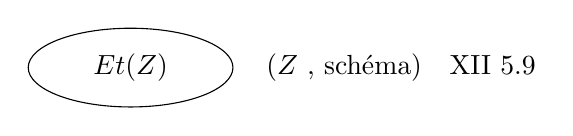
\begin{tikzpicture}
\node at (0,0) {$\operatorname{Et}(Z)$};\draw (0,0) ellipse (1.3cm and .5cm);
\node[anchor=west] at (1.6,0) {($Z$ , schéma)\quad XII 5.9};
\end{tikzpicture}}

Chow (lemme de - )\quad Chow lemma\quad XII 7.1

\deleted{Lemme de Chow}

Théorème de finitude \deleted{pour un morphisme propre\quad finiteness \unsure{theorm|theorem} for}\inserted{finiteness theorem}\quad \handwritten{$\overline{\underline{\mathrm{XIV}}}$ 1.1, \deleted{\unsure{XVI 5.1}}\inserted{$\overline{\underline{\mathrm{XVI}}}$ 5.1, 5.2} XVII ...) \inserted{$\overline{\underline{\mathrm{XIX}}}$ 5.1}}

\deleted{\handwritten{a)} pour morphisme propre\quad XIV 1.1}

\deleted{proper morphism\quad XIV 1.1}

\deleted{\handwritten{b)} pour $R^i_{\handwritten{!}}f$\quad XVII ...}
\margin{\handwritten{$\times$}}

\deleted{\handwritten{c)} pour un morphisme de type fini de schéma excellents\quad XIX 5.1}

\figure{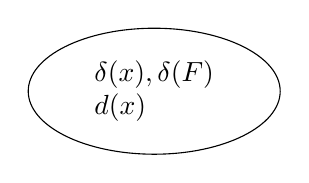
\begin{tikzpicture}
\node[align=left] at (0,0) {\inserted{\handwritten{$\delta(x),\delta(F)$}}\\$d(x)$};
\draw (0,0) ellipse (1.6cm and .8cm);
\end{tikzpicture}}
($x$, point d'un schéma\deleted{)}, \inserted{$F$ faisceau \deleted{sur $X$}}\handwritten{)}\quad \deleted{XIV (2.1)}\quad XIV 2

\inserted{\handwritten{Lefschetz}} \handwritten{(}théorème de \deleted{Lefschetz} affine\handwritten{)}\quad affine Lefschetz theorem\quad XIV 3.1 \handwritten{, XIX 6.1}

Morphisme \inserted{(universellement)} $n$-acyclique ($n$, entier)\quad \inserted{(universally)} $n$-acyclic morphisme\quad XV 1.3, 1.7

\deleted{Morphisme universellement $n$-acyclique\quad universally acyclic morphism}

\margin{\figure{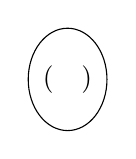
\begin{tikzpicture}\node at (0,0) {(\quad)};\draw (0,0) ellipse (.5cm and .65cm);\end{tikzpicture}}}
morphisme \inserted{(universellement\deleted{\unsure{à}})} 1-asphérique\quad \deleted{(universally)}\inserted{(universally) 1-aspheric} morphism\quad XV 1.7

\deleted{morphisme universellement 1-asphérique\quad universally 1-aspheric morphism}

Morphisme \inserted{(universellement)} localement $n$-acyclique\quad \inserted{(universally)} locally $n$-acyclic morphism\quad XV 1.11

morphisme \inserted{(universellement)} localement 1-asphérique\quad \inserted{(universally)} locally \deleted{\unsure{1}}\handwritten{1}-aspheric morphism\quad XV 1.11

\figure{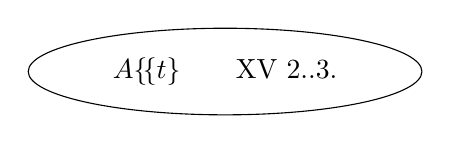
\begin{tikzpicture}
\node at (0,0) {$A\handwritten{\{\!\{}t\handwritten{\}}$\qquad XV 2\deleted{\unsure{.}}.3.};
\draw (0,0) ellipse (2.5cm and .55cm);
\end{tikzpicture}}

théorème de changement de base par morphisme lisse\quad base change theorem \deleted{for} \unsure{for|bor} smooth base change\quad XVI 1.2

théorème de spécialisation pour la cohomologie\quad speciali\deleted{\unsure{s}}zation theorem for cohomology\quad XVI 2.2

théorème de pureté cohomologique relatif\quad relative purity theorem for cohomology\quad XVI 3.6, \inserted{3.7}

théorème de pureté cohomologique absolue\quad absolute purity theorem for cohomology\quad XVI 3.9,XIX \inserted{1.2,2.1,3.2}

couple lisse \inserted{de schémas relatifs}\quad smooth pair of relative schemes\quad XVI 3.1

\deleted{Lemme} Abhyankar (lemme d'\deleted{\unsure{A}} - relatif )\quad relative \unsure{Anhyankar|Abhyankar}'s lemma\quad XVI 3.5

théorème de comparaison pour les schémas algébriques sur $\underline{C}$\quad comparison theorem for algebraic schemes over $\underline{C}$\quad XVI 4.1
% archive sheet number: 43
